\subsection{System design}
% metatext
The rideshare solution is designed to consist of multiple parts.
This section contains descriptions of the different parts, and a definition of their responsibilities.

% Description of the solution
\begin{figure}[h]
	\centering
	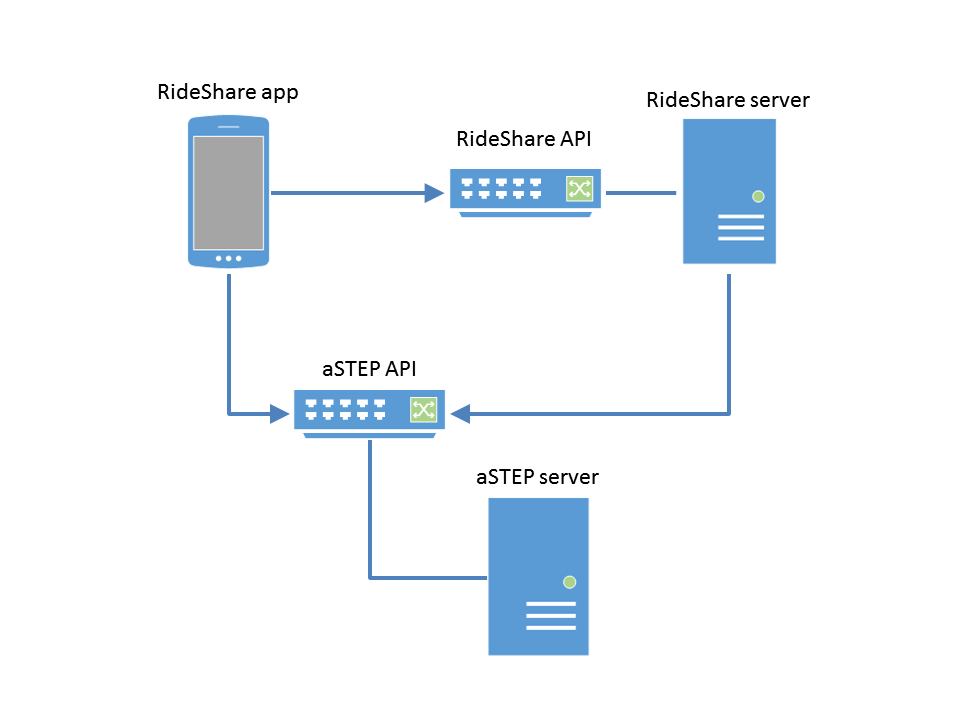
\includegraphics[width=\textwidth]{figures/SystemDesign.png}
	\caption{System design, including all major parts of the solution.}
	\label{fig:s2systemdesign}
\end{figure}

% Definition of APP responsibilities
The app...
Fetch route matches

% user management responsibilities
User interface for logging in, registering a new user, edit contact information.
Through RideShare server.

% location responsibilities
Provide aSTEP system with location data directly.



% Definition of RIDESHARE(TM) server responsibilities
RideShare server..

% user management responsibilities
Relay login request from app, save and relay the token.
Because the user management in aSTEP does not provide anything but username and password, the contact information and other data is stored on the RideShare server.


% location responsibilities
Fetch route matches for each user and store.



% Definition of aSTEP system responsibilities
aSTEP...

% user management responsibilities
Authenticate user by password.

% location responsibilities
Store locations, find stable routes, find route matches.
